\chapter{Repetitive Learning Model Predictive Control}
This chapter gives a general introduction to the concept of Model Predictive Control (MPC). Based on that, the theory of Learning Model Predictive Control (LMPC) for periodic/repetitive tasks is presented. %Additionally, simulations of LTI systems are performed and analyzed to verify its practicability.

\section{Model Predictive Control}
Model Predictive Control is a concept that has been developed since the late 1970s, starting from Chemical Process Industries \cite{garcia1989model}. Since then, increasing computational power which is essential to quickly solving complex optimization problems has helped further research on this method and has extended it to other fields beyond chemical industries.
%One strong advantage of MPC is its ability to include state and input constraints 
This section gives a brief overview on the mathematical concepts of MPC \cite{Borrelli2003}.\\
Given the discrete time system
\begin{equation}
\bm{x}_{t+1}=f(\bm{x}_t,\bm{u}_t),
\end{equation}
where $\bm{x}\in \mathbb{R}^n$ and $\bm{u}\in\mathbb{R}^m$ are the system state and input, subject to the constraints
\begin{equation}
\bm{x}_t\in\mathcal{X},\ \bm{u}_t\in\mathcal{U},\ \forall t\in\mathbb{Z}_{0+}.
\end{equation}
The MPC controller tries to minimized the following \emph{objective function} 
\begin{equation}
J_{0\rightarrow N}(\bm{x}_0,U_{0\rightarrow N})=\sum_{k=0}^{N-1}h(\bm{x}_k,\bm{u}_k) + p(\bm{x}_N)
\end{equation}
where $N$ is the time horizon. The terms $h(\bm{x}_k,\bm{u}_k)$ and $p(\bm{x}_N)$ are referred to as \emph{stage cost} and \emph{terminal cost}, respectively. 
{\bfseries{If you wanna be formal look Borrelli's book or the paper about LMPC, you need to define the optimal trajectory at time $t$ and then that you apply just the first input of that trajectory.}} {\bfseries{Also, the equations should be centered}}
Then, at each time step $t$, the objective function is minimized and its first optimal input $\bm{u}_0$ is applied to the system. This results in a Constrained Finite Time Optimal Control (CFTOC) problem:
\begin{equation}\label{eq:generalMPC}
J_{0\rightarrow N}^*(\bm{x}_0,U_{0\rightarrow N})=\min_{U_{0\rightarrow N}}\left[\sum_{k=0}^{N-1}h(\bm{x}_k,\bm{u}_k) + p(\bm{x}_N)\right]
\end{equation}
There are different approaches on how this optimization problem is solved, two common ways are the \emph{Batch Approach} and the \emph{Recursive Approach}. In general, the optimization problem is nonconvex.\\
Solving eq. \ref{eq:generalMPC} and applying the first optimal input at every time step results in a \emph{Receding horizon controller (RHC)}.

\section{Learning Model Predictive Control}\label{sec:LMPC}
Learning Model Predictive Control (LMPC) is a novel control theory that allows to find an optimal trajectory in an iterative task by learning from previous iterations. It is based on the concept of Iterative Learning Control (ILC). ILC is a control strategy {\bfseries{there are many different ILCs}} that minimizes the tracking error of an iterative process by improving its trajectory with every iteration, learning from previous trajectories. It is limited to fixed time processes with given tracking references. \cite{Lee2007} gives an overview on existing methods on ILC.\\
LMPC extends the framework of ILC by adding an optimization function which allows finding an optimal trajectory of optimal duration. Applying this strategy makes it possible to gradually find an optimal trajectory for complex nonlinear systems under only low computational cost {\bfseries{Again, this under low computational cost is a strong statement, in theory you should solve a Mixed Integer Programming Problem (The relaxation is coming but it is not there yet)}}.{\bfseries{In general if you expect people  to be tough on you then you must be able to motivate every single work that you say/write}}\\
\emph{Definition of iterative processes}\\
There are two types of iterative processes that have to be distinguished: \emph{Batch processes} and \emph{Continuous repetitive processes} \cite{Wang2009}. Batch processes are intermittently run and are usually modeled starting from the same initial state. As opposed to that, continuous repetitive processes transition directly from one iteration to the next one, meaning that the last state of an iteration matches the initial state of the next iteration.
\paragraph{Theory of LMPC}
Following theory has been adapted from \cite{Rosolia2016}.\\
First, we define the stage cost of a state $\bm{x}_t^j$ at time $t$ in iteration $j$ as follows:
\begin{equation}
h(\bm{x}_F,0)=0\text{ and } h(\bm{x}_t^j,u_t^j)>0\ \forall\ \bm{x}_t^j\in\mathbb{R}^n\setminus \{\bm{x}_F\},\bm{u}_t^j\in\mathbb{R}^m\setminus\{0\}
\end{equation}
where $\bm{x}_F$ is the final state with $f(\bm{x}_F,0)=0$.
Then, the cost of one iteration $j$ is defined as the sum of its stage costs:
\begin{equation}
J^j = J_{0\rightarrow\infty}^j(\bm{x}_0^j)=\sum_{k=0}^\infty h(\bm{x}_k^j,\bm{u}_k^j).
\end{equation}
Similarly, the cost-to-go of one specific state $\bm{x}_t^j$ of iteration $j$ is defined as
\begin{equation}\label{eq:LMPC_costToGo}
J_{t\rightarrow\infty}^j(\bm{x}_t^j)=\sum_{k=t}^\infty h(\bm{x}_k^j,\bm{u}_k^j).
\end{equation}
LMPC constructs a sampled safe set of feasible trajectories which is used as a terminal state constraint in the MPC formulation:
\begin{equation}
\mathcal{SS}^j = \left\{ \bigcup_{i\in M^j} \bigcup_{t=0}^\infty \bm{x}_t^i\right\}
\end{equation}
with
\begin{equation}
M^j=\left\{ k\in [0,j]: \lim_{t\rightarrow\infty}\bm{x}_t^k=\bm{x}_F\right\}.
\end{equation}
Additionally, a terminal cost function is defined over the sampled safe set:
\begin{equation}
Q^j(\bm{x})=\begin{dcases}
\min_{(i,t)\in F^j(\bm{x})} J_{t\rightarrow\infty}^i(\bm{x}),&\text{if }\bm{x}\in\mathcal{SS}^j\\
+\infty,&\text{if } \bm{x}\not\in \mathcal{SS}^j
\end{dcases}
\end{equation}
with
\begin{equation}
F^j(\bm{x})=\left\{(i,t):i\in [0,j],t\geq 0\text{ with }\exists\ \bm{x}_t^i\in\mathcal{SS}^j \text{ and }\bm{x}_t^i=\bm{x}\right\}.
\end{equation}
Using the terminal constraints and terminal cost we can write the finite time constrained optimal control problem:
\begin{subequations}
\begin{align}
J_{t\rightarrow t+N}^{\scalebox{0.4}{LMPC},j}(\bm{x}_t^j)&=\min_{\bm{u}_{t|t},...,\bm{u}_{t+N-1|t}}\left[\sum_{k=t}^{t+N-1}h(\bm{x}_{k|t},u_{k|t})+Q^{j-1}(\bm{x}_{t+N|t})\right]\\
\text{s.t.}\\
\bm{x}_{k+1|t}&=f(\bm{x}_{k|t},\bm{u}_{k|t}),\forall k\in[t,...,t+N],\\
\bm{x}_{t|t}&=\bm{x}_t^j,\\
\bm{x}_{k|t}&\in\mathcal{X},\bm{u}_k\in\mathcal{U},\forall k\in[t,...,t+N],\\
\bm{x}_{t+N|t}&\in\mathcal{SS}^{j-1}.
\end{align}\label{eq:generalLMPC}
\end{subequations}
It can be shown that this control strategy is recursively feasible and {\bfseries{that equuilibrium $x_F$ is asymptotically stable for the closed-loop  system (Equation of system) and (equation of controller)}}. Additionally, the iteration cost $J^j$ does not increase with the iteration index $j$ and the trajectory converges to a local optimum for $j\rightarrow\infty$.\\
The LMPC strategy presented above applies for batch processes, i.e. the initial state $x_0^j$ has to be the same for each iteration. However, it is not applicable for continuous repetitive systems, for which the final state of an iteration corresponds to the initial state of the next iteration. The next section shows the extension for the repetitive case.

\section{Repetitive Learning Model Predictive Control}
This section presents a learning control strategy for continuous repetitive systems. We prove ... using the mathematical tools we introduced in section \ref{sec:LMPC}.\\
\paragraph{Not-so-mathematical description of the proving strategy:}
Use two consecutive laps, stacked together, for the safe set and cost function.\\
Start by constructing a safe set consisting of laps 0 and 1 in which initial and final states are equal (path following). Then start lap 2 and use this safe set and its Q function. At the end of lap 2, the controller can predict beyond the finish line, into the safe set of lap 1. After the finish line has been reached and the laps have been switched (from lap 2 to lap 3), we can use the stacked safe set of laps 0+1 and laps 1+2. However, the initial state is not necessarily the same as before.\\
This idea of stacking safe sets and Q functions is presented below.
\paragraph{Periodicity and switching condition} First, we assume that the state dynamics and stage cost are periodic with periodicity vector $\bm{p}$:
\begin{align}
f(\bm{x}_k+\bm{p},\bm{u}_k) &= f(\bm{x}_k,\bm{u}_k)+\bm{p}\\
h(\bm{x}+\bm{p},\bm{u}) &= h(\bm{x},\bm{u}).
\end{align}
If the dynamics are periodic in one state, the periodicity is expressed using a standard basis vector $\bm{p}=P\bm{e}_i$, where $P$ is the periodicity in state $i$.\\
The switching from one iteration to the next one happens when the periodic state reaches $P$, i.e. $\bm{xe}_i^T\geq P$.\\
Continuous repetitive systems are defined by smooth transitions between two iterations, i.e. the final state of one iteration becomes the initial state of the following iteration. This implicates that, at the end of one iteration, the control needs to take the beginning of the next iteration into account in order to find an optimal input.\\
We achieve this by creating a safe set that extends beyond the final state of one iteration to the end of the consecutive iteration.

\paragraph{Definitions}
First, we define the stacked sampled Safe Set $\hat{\mathcal{SS}}^j$ at iteration $j$ that extends beyond the finish line (\emph{note:} it basically just contains stacks of two consecutive trajectories, e.g. laps 0+1, 1+2, 2+3, ...)
\begin{equation}
\hat{\mathcal{SS}}^j=\left\{\bigcup_{i\in M^j}\left[\left(\bigcup_{t=0}^\infty \bm{x}_t^i\right)\cup\left(\left(\bigcup_{t=0}^\infty \bm{x}_t^{i+1}\right)+\bm{p}\right)\right]\right\}
\end{equation}
with
\begin{equation}
M^j=\left\{k\in[0,j]:\lim_{t\rightarrow\infty}\bm{x}_t^{k+1}=\bm{x}_F\right\}
\end{equation}
We can also write this definition of the stacked sampled safe set as follows:
\begin{equation}
\hat{\mathcal{SS}}^j=\left\{\mathcal{SS}^j\cup \left(\mathcal{SS}^{j+1}+\bm{p}\right)\right\}
\end{equation}
% Actually, this is slightly different from the definition above since we include SS^0 in this case.
Note that this definition of the stacked sampled safe set can also be written as a function of x:
\begin{equation}\label{eq:stSafeSet}
\bm{x}\in\hat{\mathcal{SS}}^j\rightarrow
\begin{cases}
\bm{x}\in\mathcal{SS}^j&\text{if } \bm{x}<P,\\
\bm{x}\in\mathcal{SS}^{j+1}&\text{if }\bm{x}\geq P
\end{cases}
\end{equation}
Similarly to the single iteration cost-to-go from eq. \ref{eq:LMPC_costToGo}, we define the \emph{stacked cost-to-go} $\hat{J}_{t\rightarrow\infty}^j(\bm{x}_t^j)$ of iteration $j$ as follows:
\begin{equation}
\hat{J}_{t\rightarrow\infty}^j(\bm{x}_t^j)=\begin{dcases}
J_{t\rightarrow\infty}^j(\bm{x}_t^j)+J^{j+1}&\text{if } \bm{x}<P,\\
J_{t\rightarrow\infty}^{j+1}(\bm{x}_t^{j+1})&\text{if } \bm{x}\geq P
\end{dcases}
\end{equation}
\emph{Note:} the stacked cost-to-go is a piecewise defined function, it is continuous through the lap switching condition (at $P$) and it is zero at $2P$. It is illustrated in fig. \ref{fig:stackedCostToGo}.\\
\begin{figure}[ht]
    \centering
  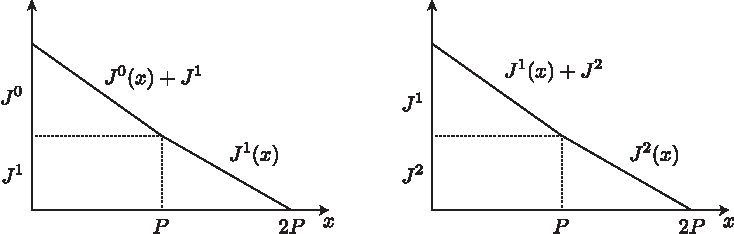
\includegraphics{../../figures/Illustrator/proof3.pdf}
    \caption{Stacked cost-to-go $\hat{J}^0$ and $\hat{J}^1$}
    \label{fig:stackedCostToGo}
\end{figure}
This stacking extends the cost-to-go beyond the finish line and allows at the end of one lap to consider the beginning of the next lap (for which the predicted $x_{t+N|t}>P$).\\
Using this definition of the stacked cost-to-go we define the stacked Q-function:
\begin{equation}
\hat{Q}^j(\bm{x})=\begin{dcases}
\min_{(i,t)\in F^j(\bm{x})} \hat{J}_{t\rightarrow\infty}^i(\bm{x}),&\text{if }x\in\hat{\mathcal{SS}}^j,\\
+\infty&\text{if }x\not\in\hat{\mathcal{SS}}^j.
\end{dcases}
\end{equation}
We can also write the stacked Q function depending on x:
\begin{equation}
\hat{Q}^j(\bm{x})=\begin{dcases}
\min_{i,t} \left[J_{t\rightarrow\infty}^i(\bm{x})+J^{i+1}\right],&\text{if }\bm{x}<P,i\in[0,j]\\
\min_{i,t} \left[J_{t\rightarrow\infty}^{i+1}(x)\right],&\text{if }\bm{x}>P,i\in[0,j].\\
\end{dcases}
\end{equation}
With these definitions, we redefine the LMPC function which yields the repetitive LMPC function:
\begin{subequations}
\begin{align}
\hat{J}_{t\rightarrow t+N}^{\scalebox{0.4}{LMPC},j}(\bm{x}_t^j)&=\min_{\bm{u}_{t|t},...,\bm{u}_{t+N-1|t}}\left[\sum_{k=t}^{t+N-1}h(\bm{x}_{k|t},u_{k|t})+\hat{Q}^{j-2}(\bm{x}_{t+N|t})\right]\\
\text{s.t.}\\
\bm{x}_{k+1|t}&=f(\bm{x}_{k|t},\bm{u}_{k|t}),\forall k\in[t,...,t+N],\\
\bm{x}_{t|t}&=\bm{x}_t^j,\\
\bm{x}_{k|t}&\in\mathcal{X},\bm{u}_k\in\mathcal{U},\forall k\in[t,...,t+N],\\
\bm{x}_{t+N|t}&\in\hat{\mathcal{SS}}^{j-2}.
\end{align}\label{eq:generalRLMPC}
\end{subequations}
\emph{Note:} Since we use stacks of 2 consecutive laps for the safe set and Q function, we can't use the previous safe set $j-1$ but instead the one even further back, $j-2$. Our stacked safe set $\hat{\mathcal{SS}}^0$ also has to contain two successful laps before the LMPC starts!
\paragraph{Recursive feasibility}
Recursive feasibility throughout one iteration is guaranteed as usual. However, we have to prove feasibility even through the switching between two laps.\\
Consider state $\bm{x}_t^j$ in iteration $j$. Then the terminal constraint enforces $\bm{x}_{t+N|t}^{*,j}\in\hat{\mathcal{SS}}^{j-2}$. Assume that $\bm{x}_t^j$ is the last state of iteration $j$, meaning that $\bm{x}_{t+1|t}^{*,j}\geq P$ and therefore $\bm{x}_{t+N|t}^{*,j}\geq P$.\\
Using the definition of the stacked safe set in eq. \ref{eq:stSafeSet} leads to $\bm{x}_{t+N|t}^{*,j}\in\mathcal{SS}^{j-1}$.\\
As before, the state update and prediction are assumed identical, leading to
\begin{equation}
\bm{x}_{t+1|t}^{*,j}=\bm{x}_{t+1}^j=\bm{x}_{0}^{j+1}
\end{equation}
% note, actually, we're ignoring the periodicity vector p here! How can this be handled best, mathematically?
In iteration $j+1$ we use the the stacked safe set $\hat{\mathcal{SS}}^{j-1}$ with $\bm{x}<P$, leading to $\bm{x}\in\mathcal{SS}^{j-1}$. This means that the state trajectory
\begin{align}
\begin{pmatrix}
x_{t+1|t}^{*,j}, & x_{t+2|t}^{*,j}, &...,&x_{t+N-1|t}^{*,j}, &x_{t^*|t}^{i^*}, &x_{t^*+1|t}^{i^*}
\end{pmatrix}
=\\
\begin{pmatrix}
x_{0|t}^{*,j+1}, & x_{1|t}^{*,j+1}, &...,&x_{N-2|t}^{*,j+1}, &x_{t^*|t}^{i^*}, &x_{t^*+1|t}^{i^*}
\end{pmatrix}
\end{align}
is still feasible in iteration $j+1$.
\paragraph{Asymptotic stability}
The proof for asymptotic stability within an iteration works as in the standard LMPC case.
As usual, we can show that $J_{0\rightarrow N}^{\scalebox{0.4}{LMPC},j}(x_t^j)$ is a decreasing Lyapunov function in lap $j$ and we can show that $J_{0\rightarrow N}^{\scalebox{0.4}{LMPC},j+1}(x_t^j)$ is a decreasing Lyapunov function in lap $j+1$.
However, we are interested in the stability when the lap switching happens. Looking at the LMPC cost at the state at the switching condition shows an incontinuity.\\
Consider state $\bm{x}_t^j=\bm{x}_0^{j+1}$ as the last state of iteration $j$ and the first state of iteration $j+1$. 
\begin{align}
J_{0\rightarrow N}^{\scalebox{0.4}{LMPC},j}(x_t^j)&=\min_u\left[\sum_{k=0}^{N-1}h(x_{k|t},u_{k|t})+\hat{Q}^{j-2}(x_{N|t})\right] & \text{and } x_{N|t}>P\\
&=\min_u\left[\sum_{k=0}^{N-1}h(x_{k|t},u_{k|t})+Q^{j-1}(x_{N|t})\right]\\
&=\min_u\left[\sum_{k=0}^{N-1}h(x_{k|t},u_{k|t})+\min_{i,t} \left[J_{t\rightarrow\infty}^i(x)\right]\right] & \text{and } i\in [0,j-1]\\
J_{0\rightarrow N}^{\scalebox{0.4}{LMPC},j+1}(x_0^{j+1})&=\min_u\left[\sum_{k=0}^{N-1}h(x_{k|0},u_{k|0})+\hat{Q}^{j-1}(x_{N|0})\right] & \text{and } x_{N|0}<P\\
&=\min_u\left[\sum_{k=0}^{N-1}h(x_{k|0},u_{k|0})+\min_{i,t} \left[J_{t\rightarrow\infty}^i(x)+J^{i+1}\right]\right] & \text{and } i\in [0,j-1]
\end{align}
and therefore
\begin{equation}
J_{0\rightarrow N}^{\scalebox{0.4}{LMPC},j+1}(x_0^{j+1})\geq J_{0\rightarrow N}^{\scalebox{0.4}{LMPC},j}(x_t^j).
\end{equation}
This result essentially just shows that the LMPC cost at the initial state of lap $j+1$ is larger or equal to the LMPC cost at the same state, but evaluated in the previous lap $j$.\\
Question: Can we still assume stability through iterations since the cost function is stable all the way \emph{to} the switching condition and it is stable starting \emph{from} the switching condition?
\paragraph{Non decreasing iteration cost} Using the strategy above, we will have to focus on the transition between two laps. The "problem" is that - at the beginning of an iteration, right after the transition - the controller doesn't even notice that laps were switched. The safe set is the same and the Q function only increased by a constant value.
% Explain concept of going to 2*P
% Define J (not to infinity but only to P)
% Define stacked Q and the two areas (< P and >P)
% Prove feasibility
% Show and discuss stability/non increasing cost